\documentclass[conference]{IEEEtran}
\IEEEoverridecommandlockouts
% The preceding line is only needed to identify funding in the first footnote. If that is unneeded, please comment it out.
\usepackage{cite}
\usepackage{amsmath,amssymb,amsfonts}
\usepackage{algorithmic}
\usepackage{graphicx}
\usepackage{textcomp}
\usepackage{xcolor}
\usepackage{subcaption}
\usepackage[colorlinks=false]{hyperref}
\hypersetup{
    hidelinks
}
\definecolor{til}{HTML}{1E8449}
\definecolor{maxim}{HTML}{6C3483}
\definecolor{baptiste}{HTML}{21618C}

\def\BibTeX{{\rm B\kern-.05em{\sc i\kern-.025em b}\kern-.08em
    T\kern-.1667em\lower.7ex\hbox{E}\kern-.125emX}}
\begin{document}

\title{Statistical Machine Learning Final Project\\
    {\large solved with Random Forest and SVM}
}

\author{\IEEEauthorblockN{1\textsuperscript{st} Tilman Marquart}
\IEEEauthorblockA{\textit{Computer Science Bachelor} \\
\textit{SDU Exchange Student}\\
Nuremberg, Germany \\
timar20@student.sdu.dk \\
\color{til}{written text will appear in green}}
\and
\IEEEauthorblockN{2\textsuperscript{nd} Maxime Gatineau}
\IEEEauthorblockA{\textit{Engineering Master} \\
\textit{SDU Exchange Student}\\
Lille, France \\
magat20@student.sdu.dk \\
\color{maxim}{written text will appear in purple}}
\and
\IEEEauthorblockN{3\textsuperscript{rd} Baptiste Piofret}
\IEEEauthorblockA{
\textit{SDU Exchange Student}\\
Versailles, France \\
bapio20@student.sdu.dk \\
\color{baptiste}{written text will appear in blue}}
}

\maketitle

\begin{abstract}
final project abstract, use random forest and ...
maybe write some intro sentences about the problem we try to solve
\end{abstract}

\section{Introduction}
%Give a brief intuitive summary of the two chosen classification algorithms. Identify the critical parameters.
%Talk about random forest with PCA. => critical hyperparams: PCA, NTREE, MTRY, NODESIZE, SAMPSIZE
\textcolor{til}{
    Our overall goal was to choose one fast but not so precise algorithm and one slower but more precise algorithm. We interpret fast as low training and prediction time. To choose the right algorithm we took a look at the asymptotic time complexity of the statistical machine learning algorithms (Table \ref{table:timeComplexity}).}

\textcolor{til}{
    For the fast but not so precise algorithm we choosed Random Forest. In addition to classical Decision Trees, will Random Forest generalize better on unseen data (important for the distinct people problem) by controlling the amount of various trees ($n_{trees}$). At the same time $n_{trees}$ will have a direct influence on our training and prediction time as seen in Table \ref{table:timeComplexity}, so we have to find a good balance for this hyper parameter. Other critical hyper parameters for Random Forest are: The amount of input features ($p$); Amount of features tried ($m_{try}$); Nodesize (${nodesize}$) controlling the tree depth; And lastly the sample size (${sampsize}$). We will discuss them in detail in Section \ref{sec:hyper:rf}.}

\textcolor{maxim}{
    For the slower but more precise method we decided to use a Support Vector Machine (SVM).
    Insert explanation of SVM here and a brief statement why.
}
\textcolor{maxim}{
    Critical hyper parameters for Support Vector Machine are: The type of Kernel used ($K_{type}$); The amount of Principal Components ($p$); The Cost ($C$); And lastly, the parameter of the Kernel ($K_{par}$).
}

% \begin{itemize}
%     \item The amount of features ($p$) which we try to reduce with a PCA preprocessing.
%     \item Amount of features tried ($m_{try}$) for finding the best decision point for the new tree branch.
%     \item Nodesize controls the minimum amount of samples in the leaf nodes and therefore also controls the depth of the tree.
% \end{itemize}

%ntree over classical dec. tree because it seems to be more robust against overfitting on just train part because of the parallel generated random trees.

\begin{table}[htbp]
    \color{til}
    \caption{\color{til}Time complexity in Big-O-Notation}
    \begin{center}
    \begin{tabular}{|c|c|c|}
        \hline
        \textbf{Algorithm} & \textbf{Training} & \textbf{Prediction} \\
        \hline
        Decision Tree & $\mathcal{O}(n^2p)$ & $\mathcal{O}(p)$ \\
        \hline
        Random Forest & $\mathcal{O}(n^2pn_{trees})$ & $\mathcal{O}(pn_{trees})$ \\
        \hline
        Support Vector Machine & $\mathcal{O}(n^2p+n^3)$ & $\mathcal{O}(n_{sv}p)$ \\
        \hline
        k-Nearest Neighbors & - & $\mathcal{O}(np)$ \\
        \hline
        \multicolumn{3}{l}{$n$ size of training dataset, $p$ number of features used } \\
        % \multicolumn{4}{l}{$p$ number of features used } \\
        \multicolumn{3}{l}{$n_{trees}$ number of various trees, $n_{sv}$ number of support vectors } \\
        % \multicolumn{4}{l}{$n_{sv}$ number of support vectors }
    \end{tabular}
    \label{table:timeComplexity}
    \end{center}
\end{table}

\begin{figure}[htbp]
    \centerline{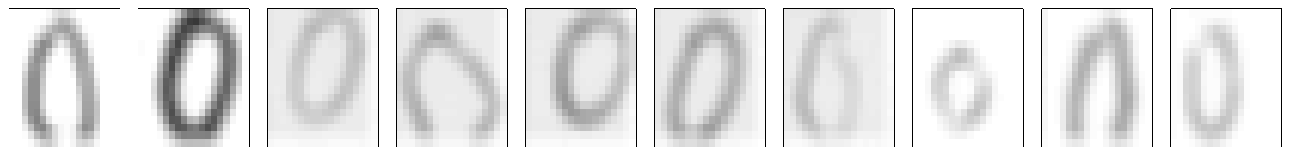
\includegraphics[width=1.0\linewidth]{preprocessing/mid_withoutNorm.pdf}}
    \centerline{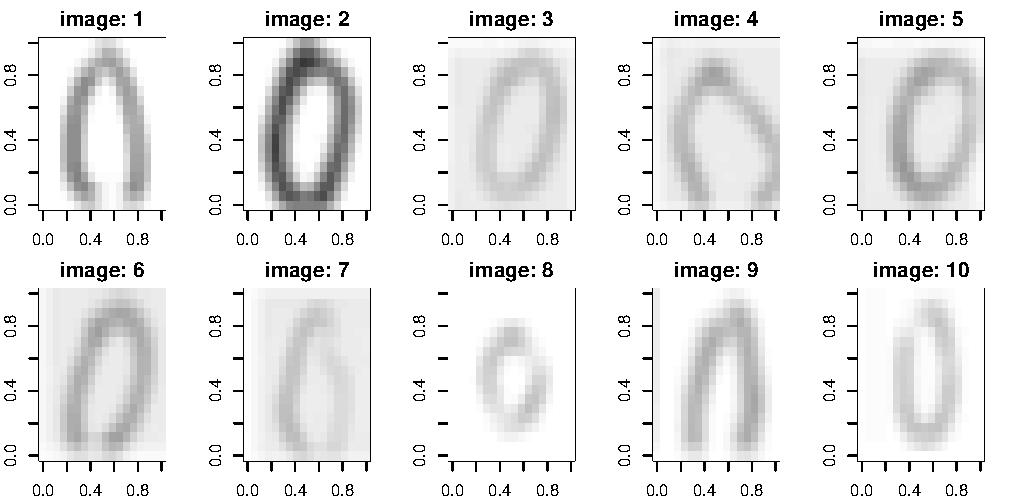
\includegraphics[width=1.0\linewidth]{preprocessing/corner_withoutNorm.pdf}}
    \centerline{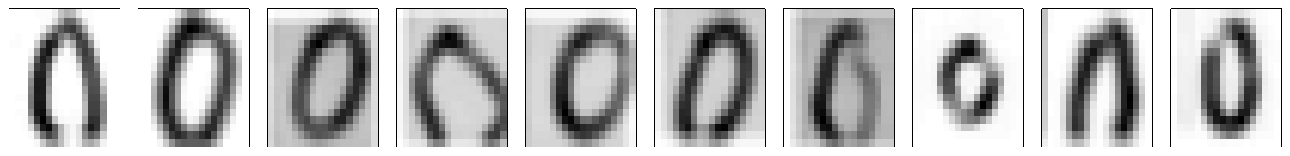
\includegraphics[width=1.0\linewidth]{preprocessing/corner_withNorm.pdf}}
    \caption{\color{til}Zero digits from first 10 students (left to right) in 100dpi mid dataset in first row; The same with the corner dataset in second row; Image wise min-max-normalization of corner dataset in third row}
    \label{fig:dataset}
\end{figure}

\begin{figure*}[ht!]
    \centering

    \subfloat[][]{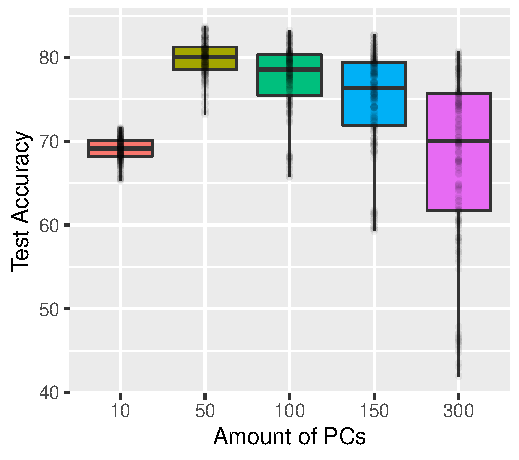
\includegraphics[width=0.3201\linewidth]{RandomForest/hypergrid/plots/final_run_28052020_pca_acc_barplot.pdf}}\quad
    \subfloat[][]{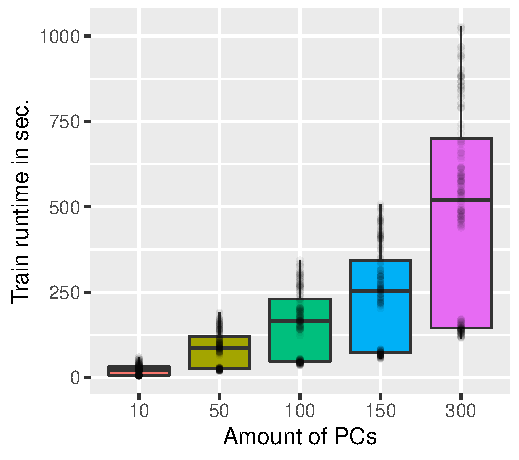
\includegraphics[width=0.3201\linewidth]{RandomForest/hypergrid/plots/final_run_28052020_pca_trainDuration_barplot.pdf}}\quad
    \subfloat[][]{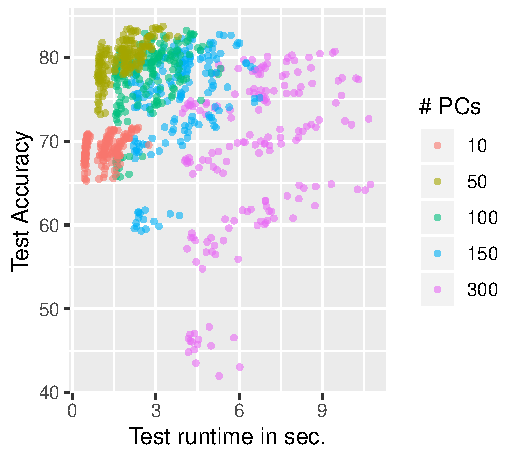
\includegraphics[width=0.3201\linewidth]{RandomForest/hypergrid/plots/final_run_28052020_pca_testDuration.pdf}}\quad

    \subfloat[][]{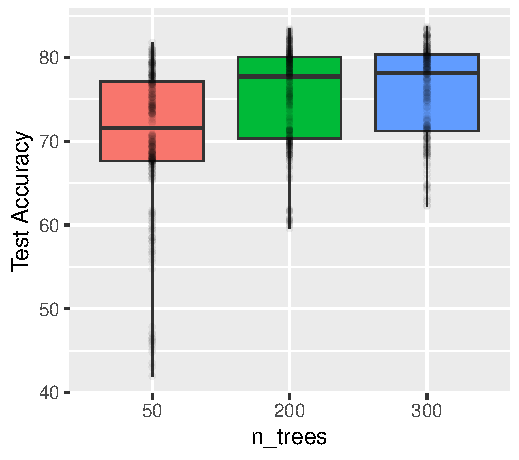
\includegraphics[width=0.3201\linewidth]{RandomForest/hypergrid/plots/final_run_28052020_ntree_acc_barplot.pdf}}\quad
    \subfloat[][]{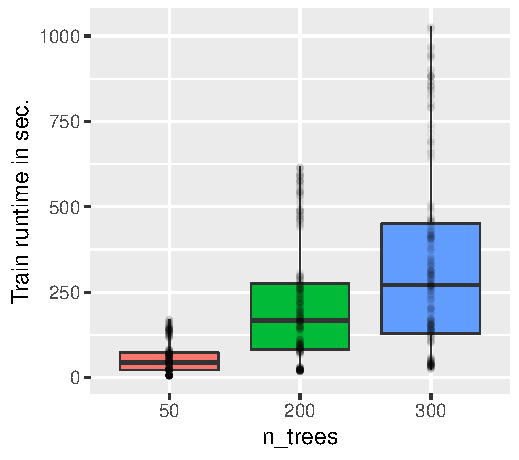
\includegraphics[width=0.3201\linewidth]{RandomForest/hypergrid/plots/final_run_28052020_ntree_trainDuration_barplot.pdf}}\quad
    \subfloat[][]{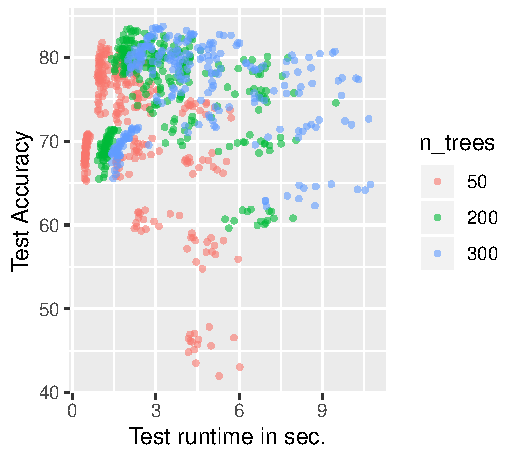
\includegraphics[width=0.3201\linewidth]{RandomForest/hypergrid/plots/final_run_28052020_ntree_testDuration.pdf}}\quad

    \caption{
        \color{til}
        Accuracy and runtime results of the 960 hyperparameter combinations; (a) Boxplot showing the accuracy for the hypergrid PCA sequence; (b) equivalent but for training runtime instead of accuracy; (c) accuracy over test runtime, ideal would be a point in the top left corner; (d,e,f) respectively to (a,b,c) but for amount of various trees $n_tree$ instead of $p$.
    }
    \label{fig:hyper:pca}
\end{figure*}

\section{Dataset and Preprocessing}
%TODO: Describe your preprocessing (dpi, PCA, centering, smoothing, normalization). Also show images. 
%TODO: why corner and not mid? => on a visual inspection corner seemed to be better centered and the digits better captured  => done
\textcolor{til}{
    During a visual inspection of the corner and mid dataset, the corner dataset seemed to better center the scanned digits and also cover the corners a bit better (See first two rows of Fig. \ref{fig:dataset}). We therefore decided to use the corner dataset for all out further analysis and the hyperparameter tuning. We later tried again the mid dataset on our tuned and optimized models and had worse results as with the corner dataset. This could proof our initial observations or more likely, the worse results are owed to the optimization of the model on the corner dataset. \\
    %TODO: why image wise min max norm? => some images with low saturation, digits probably written with a bright pencil
    While visually inspecting the dataset, we also discovered some images with low saturation, most likely these digits were written with a bright or colored pencil. In order to reduce the difference between images with high and low saturation, we apply a min-max-normalization on each image. Important to say is, that we are not using a traditional min-max-normalization with the minimum and maximum taken from the whole dataset but instead take the minimum and maximum from all 324 pixels of a single image and normalize the other pixel values with these minimum and maximum values. The result of this normalization is a dataset with equally saturated images as we can see in the third row of Fig. \ref{fig:dataset}. Especially for the disjunct problem this normalization improved the accuracy by 1,88\% for Random Forest.
}
\subsubsection{Random Forest Dataset and Preprocessing}
%TODO: why 100 dpi? => one goal was to be fast, small image size will increase fastness => done
\textcolor{til}{
    As seen in Table \ref{table:timeComplexity} the amount of features will have a direct influence on the runtime. Since we want to keep the runtime low for our Random Forest we try to reduce the amount of features with PCA beforehand. In behalf to minimize the runtime we used the dataset with 100dpi, since calculating the Principal Components will take way longer as higher the resolution of the input dataset is.
}

\subsection{Hyper parameter Optimization}
Optimize critical parameters (discussed under 1) on a smaller set and document this optimization process.

\begin{table}[htbp]
    \color{til}
    \caption{\color{til}Sequences for the hyperparameter grid}
    \begin{center}
    \begin{tabular}{|c|c|}
        \hline
        \textbf{Hyperparameter} & \textbf{Sequence} \\
        \hline
        Amount of Principal Components $p$ & 10, 50, 100, 150, 300\\
        \hline
        Random Forest $n_{trees}$ & 50, 200, 300\\
        \hline
        Random Forest $m_{try}$ & 1, 2, 4, 8\\
        \hline
        Random Forest ${nodesize}$ & 5, 20, 40, 60, 80\\
        \hline
        Random Forest ${sampsize}$ & 42000, 48000, 54000\\
        \hline
    \end{tabular}
    \label{table:hyperParamGrid}
    \end{center}
\end{table}


\begin{figure*}[ht!]
    \centering

    \subfloat[][]{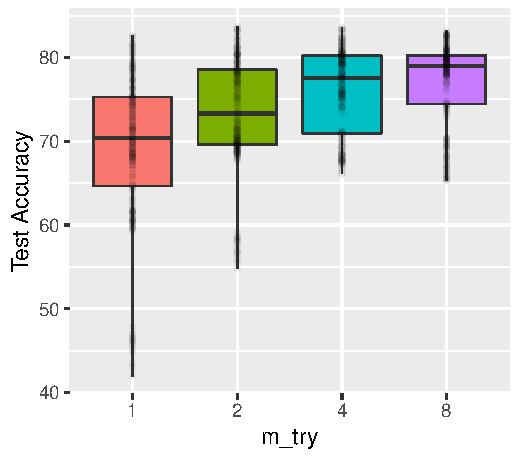
\includegraphics[width=0.3201\linewidth]{RandomForest/hypergrid/plots/final_run_28052020_mtry_acc_barplot.pdf}}\quad
    \subfloat[][]{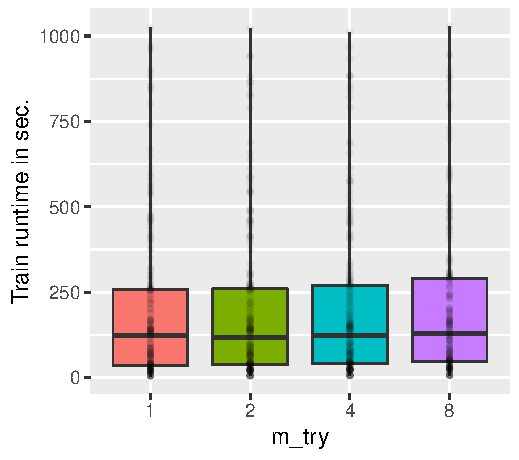
\includegraphics[width=0.3201\linewidth]{RandomForest/hypergrid/plots/final_run_28052020_mtry_trainDuration_barplot.pdf}}\quad
    \subfloat[][]{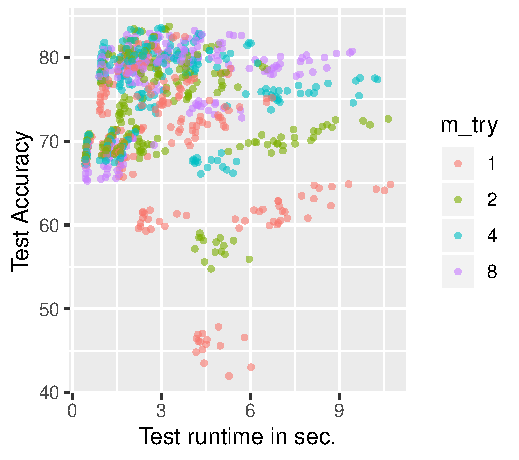
\includegraphics[width=0.3201\linewidth]{RandomForest/hypergrid/plots/final_run_28052020_mtry_testDuration.pdf}}\quad

    \subfloat[][]{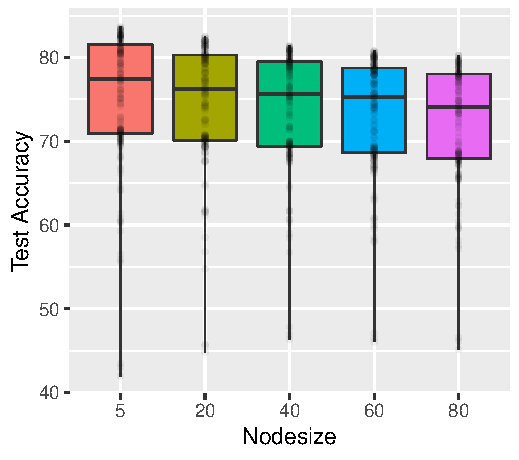
\includegraphics[width=0.3201\linewidth]{RandomForest/hypergrid/plots/final_run_28052020_nodesize_acc_barplot.pdf}}\quad
    \subfloat[][]{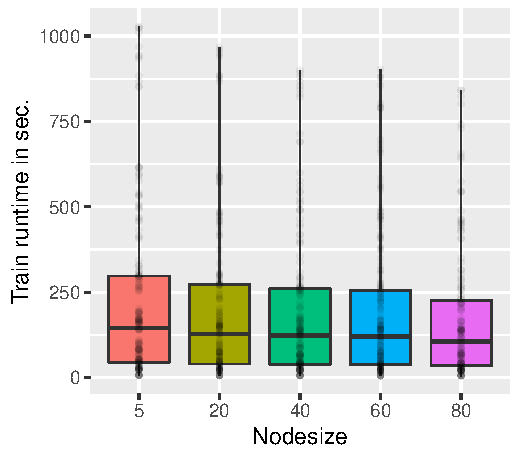
\includegraphics[width=0.3201\linewidth]{RandomForest/hypergrid/plots/final_run_28052020_nodesize_trainDuration_barplot.pdf}}\quad
    \subfloat[][]{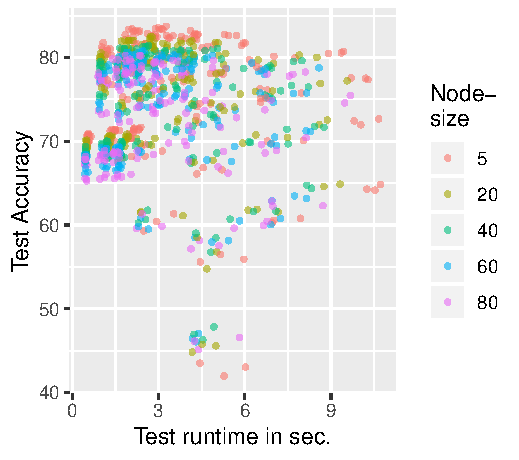
\includegraphics[width=0.3201\linewidth]{RandomForest/hypergrid/plots/final_run_28052020_nodesize_testDuration.pdf}}\quad

    \caption{
        \color{til}
        (a,b,c) respectively to Fig. \ref{fig:hyper:pca}(a,b,c) but for amount of features to try $m_{try}$ instead of $p$; (d,e,f) respectively to Fig. \ref{fig:hyper:pca}(a,b,c) but for ${nodesize}$ instead of $p$;
    }
    \label{fig:hyper:mtry}
\end{figure*}
\subsection{Hyper parameter Optimization for Random Forest}\label{sec:hyper:rf}
\textcolor{til}{
    Since optimizing random forest on the smaller dataset, was not bringing the right generalization, we decided to use a medium size dataset of 30 distinct people for training and the remaining 17 for testing and automate the finding of the right hyperparameters with a grid search. Therefore we create a hyperparameter grid with 960 combinations of the 5 hyperparameters (See Table \ref{table:hyperParamGrid} for details of the grid) and splitted them into 10 segments. We then used 4 Google Colab and 6 Kaggle notebooks in parallel, to let each segment of combinations run on each notebook. For each run we saved the Random Forest training and prediction runtime and the prediction accuracy on the test set. Google Colab and Kaggle are using nearly the same Intel Xeon CPU which was important to have a comparable runtime. In total the gridsearch took 47 hours and 53 minutes. The best result had a test accuracy of 83.72\% (See Table \ref{table:timeIntermediateResults} for further information). In the following sections we will discuss the results of the gridsearch and how we used the results for a further manual fine tuning of the hyper parameters. 
    \subsubsection{Amount of Principal Components $p$}
    The amount of features $p$ will have a direct influence on the training and testing runtime as we can see in the computational complexity $\mathcal{O}(n^2pn_{trees})$ and $\mathcal{O}(pn_{trees})$. In order to keep Random Forest fast, we use Principal Components Analysis (PCA) to reduce the amount of features and use the first $p$ Principal Components (PCs) as our $p$ input features for Random Forest. The runtime results of our hypergrid search also proof the theoretical computational complexity as we can see in Figure \ref{fig:hyper:pca}b). The highest test accuracy of our results (Figure \ref{fig:hyper:pca}a) could be achieved by taking the first 50 PCs as input features. Adding more components even decreased the accuracy, which indicates an overfitting. With 50 PCs as Input Features, performs Random Forest still very fast (around 3 seconds) while also archiving it's best accuracy for our problem (See cluster of green dots in upper left corner of Figure \ref{fig:hyper:pca}c). Hence we took the 50 PCs and manually fine tuned our model further. Finally we came up with a final value of 40 PCs for our Random Forest PCA preprocessing.
}
\textcolor{til}{
\subsubsection{Random Forest $n_{trees}$}
As we would expect it from the computational complexity and as we can see it in our test results the amount of various trees $n_{trees}$, which the Random Forest algorithm growth, heavily effects train runtime (see Fig. \ref{fig:hyper:pca}e)) as well as test runtime (see Fig. \ref{fig:hyper:pca}f)). We therefore looking for the lowest value of $n_{trees}$ which still achieves a good accuracy. As we can see in Figure \ref{fig:hyper:pca}d) the accuracy does not vary a lot between 200 or 300 Trees, so we decided on a final $n_{trees}$ value of 200, because of the faster test and train runtime.
\subsubsection{Random Forest $m_{try}$}
In Random Forest training, the amount of features tried ($m_{try}$), controls how many features are checked for finding the best decision point for a new tree branch. Therefore it has no influence on the testing time. As we can see in Figure \ref{fig:hyper:mtry}, all values of $m_{try}$ (different colors) are evenly spread along the test runtime axis which confirms this assumption. Since we reached the highest mean test accuracy at the border of our $m_{try}$ grid domain, we manually tested even higher values for $m_{try}$ for our final model, but all of the higher values had even worse results, so we finally choose a $m_{try}$ value of 4 which yielded the best test accuracy.
\subsubsection{Random Forest ${nodesize}$}
The hyper parameter ${nodesize}$ controls the minimum amount of samples in the leaf nodes and therefore also controls the depth of the tree. By decreasing this value our tree will grow deeper and therefore the test and train time will increase. We can also see the increasing train (see Fig. \ref{fig:hyper:mtry}e) and test time (slight shift of red points to the right in Fig. \ref{fig:hyper:mtry}f) in our hyper grid search results. Even if it increases test and train time we choose 5 as our final ${nodesize}$, since it brought the best accuracy (see Fig. \ref{fig:hyper:mtry}d). During manual fine tuning we tried even smaller values but had worse results, probably because of overfitting.
\subsubsection{Random Forest ${sampsize}$}
During the grid search we tried out 3 different values for ${sampsize}$. This value will define how many samples from the input data are taken into consideration to generate the decission trees. Our grid search results did not showed a significant difference in accuracy between all of the 3 tested values. We therefore decided to use the default value of this hyperparameter.
}

\begin{table}[htbp]
    \color{maxim}
    \caption{\color{maxim}Sequences for the hyperparameter grid}
    \begin{center}
    \begin{tabular}{|c|c|}
        \hline
        \textbf{Hyperparameter} & \textbf{Sequence} \\
        \hline
        Kernel Type $K_{type}$ & vanilladot, rbfdot, polydot,\\ 
        & tanhdot, laplacedot, besseldot\\
        \hline
        Amount of Principal Components $p$ & 25, 40, 50, 60, 75, 100, 150, 200\\
        \hline
        Cost $C$ & 3^{-4}, 3^{-2}, 1, 3^2, 3^4, 3^8, 3^{12}\\
        \hline
        Kernel Parameter $K_{par}$ & "automatic", "manual"\\
        \hline
    \end{tabular}
    \label{table:gridParamSVM}
    \end{center}
\end{table}


\begin{figure*}[ht!]
    \centering

    \subfloat[][]{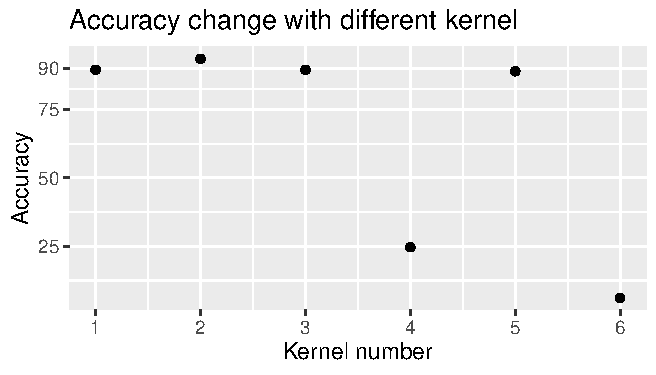
\includegraphics[width=0.3201\linewidth]{finalProject/SVM/Images_small/AllIn_Accuracy_Kernel.pdf}}\quad
    \subfloat[][]{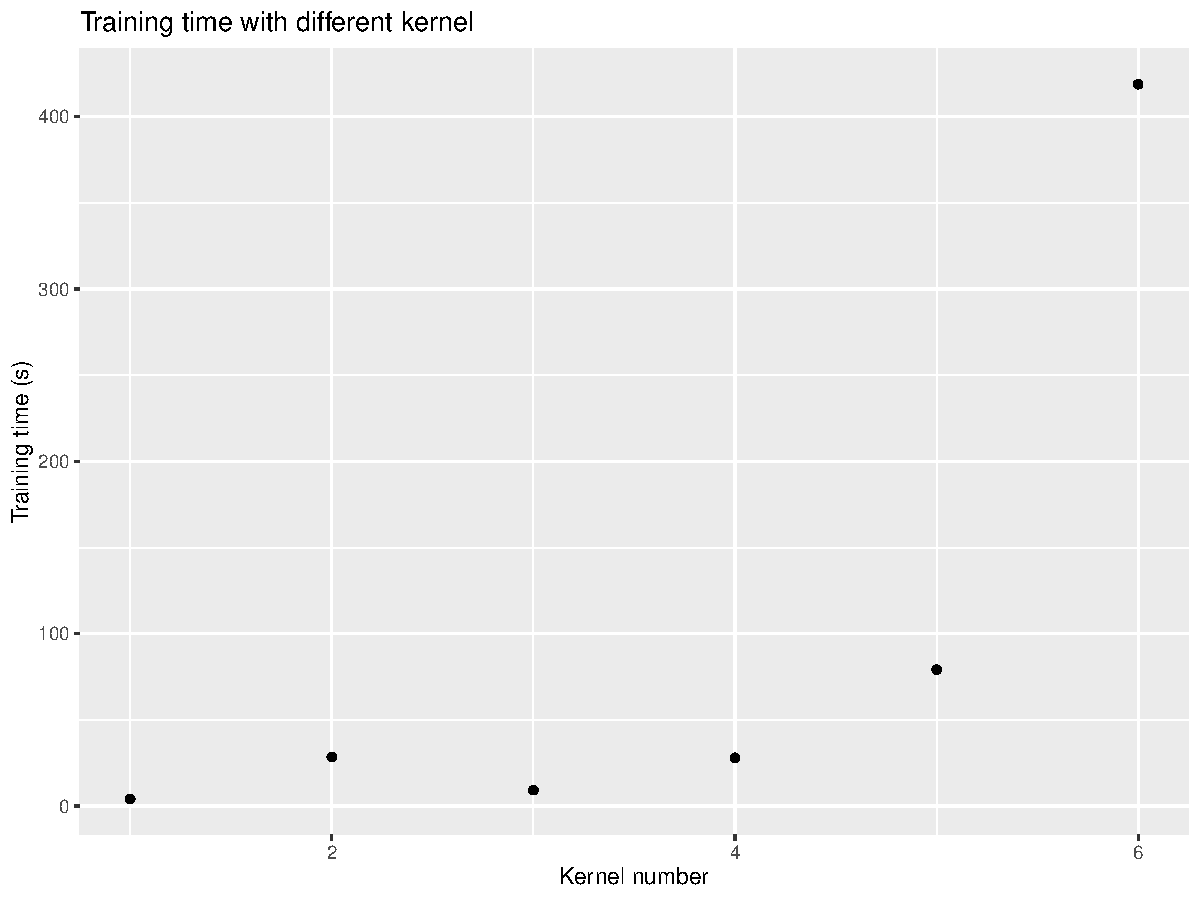
\includegraphics[width=0.3201\linewidth]{finalProject/SVM/Images_small/AllIn_Training_Kernel.pdf}}\quad
    \subfloat[][]{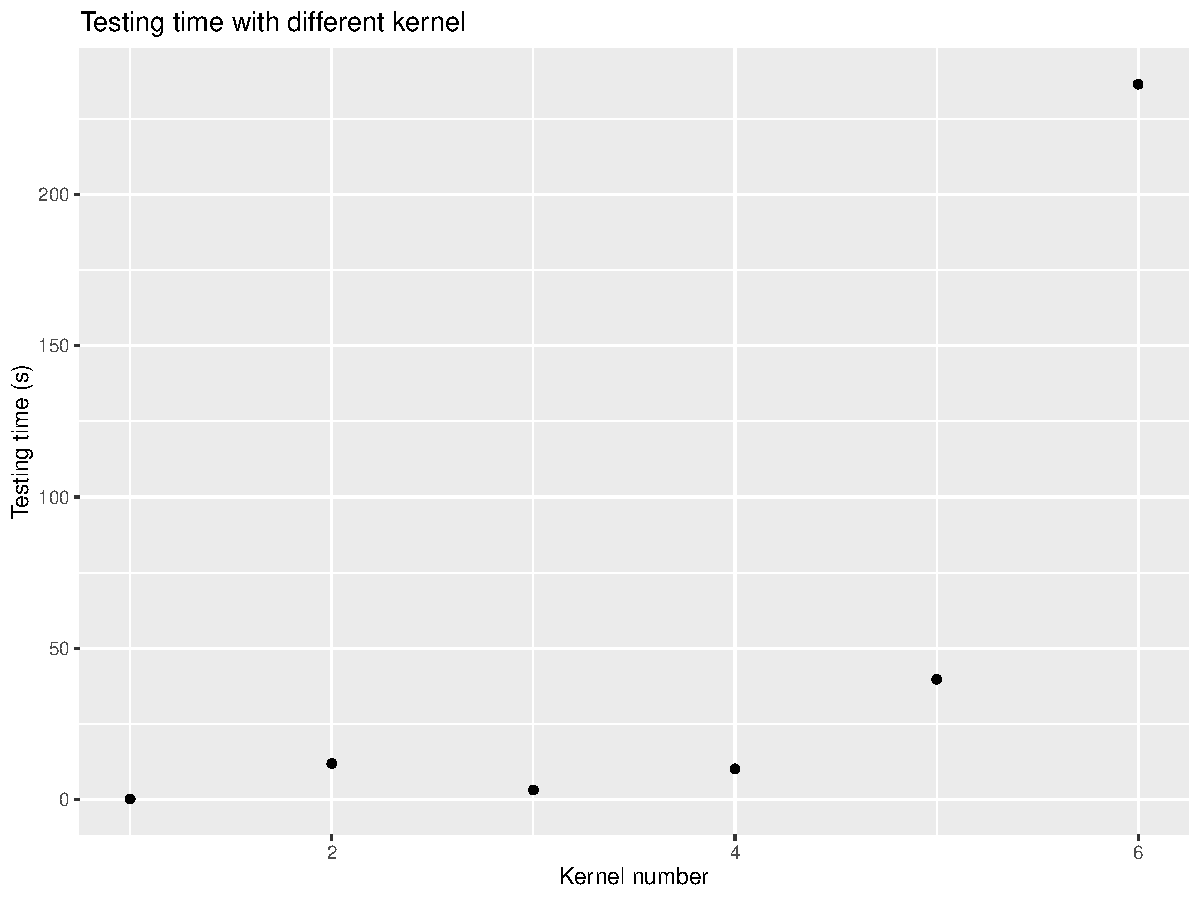
\includegraphics[width=0.3201\linewidth]{finalProject/SVM/Images_small/AllIn_Testing_Kernel.pdf}}\quad
    
     \subfloat[][]{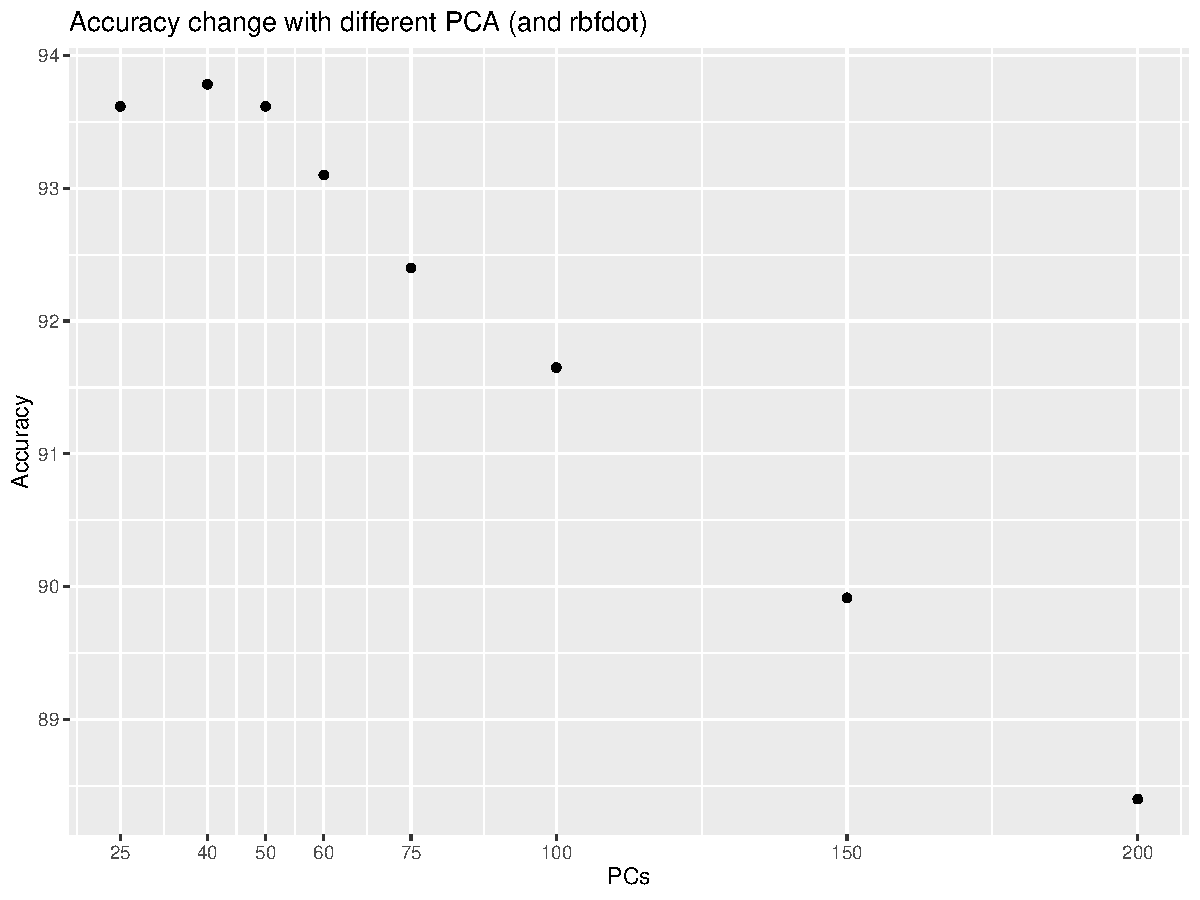
\includegraphics[width=0.3201\linewidth]{finalProject/SVM/Images_small/AllIn_Accuracy_PCA.pdf}}\quad
    \subfloat[][]{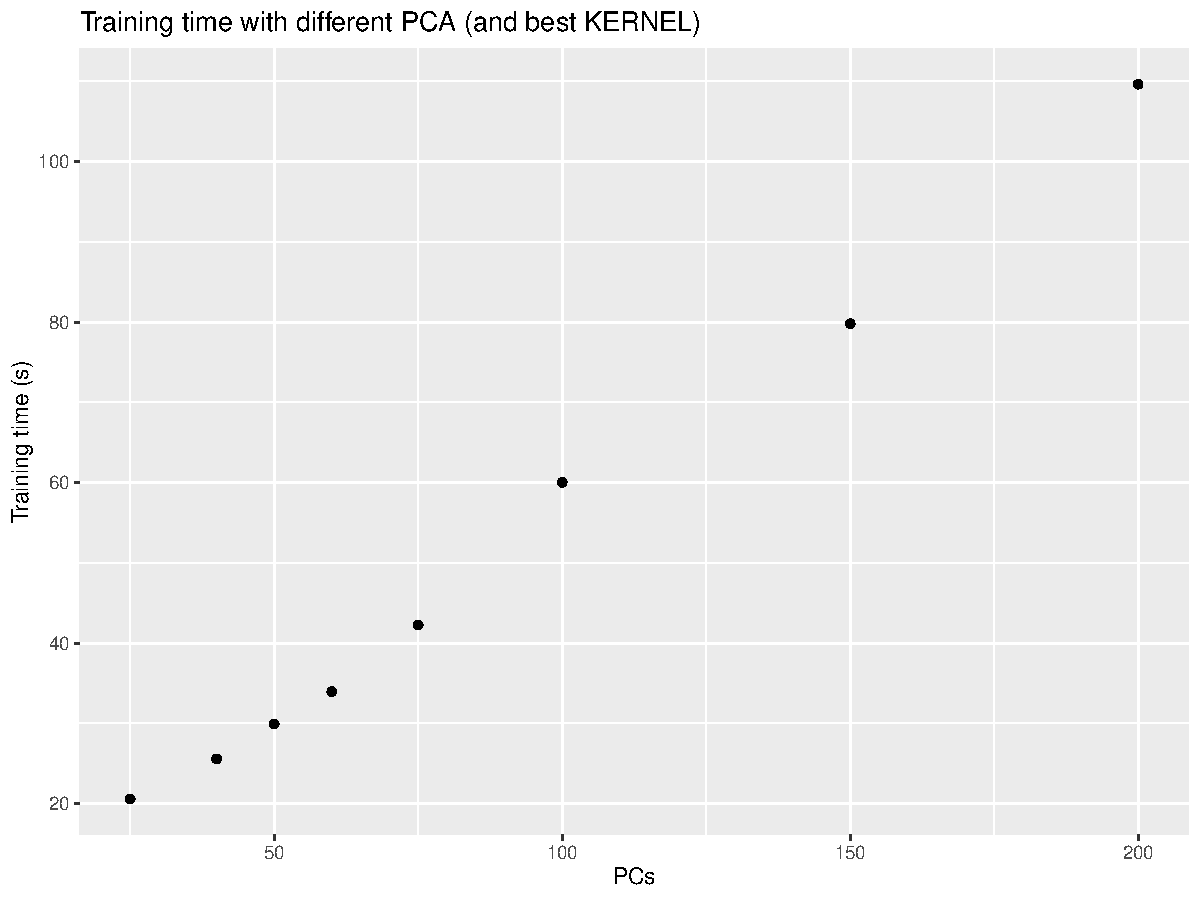
\includegraphics[width=0.3201\linewidth]{finalProject/SVM/Images_small/AllIn_Training_PCA.pdf}}\quad
    \subfloat[][]{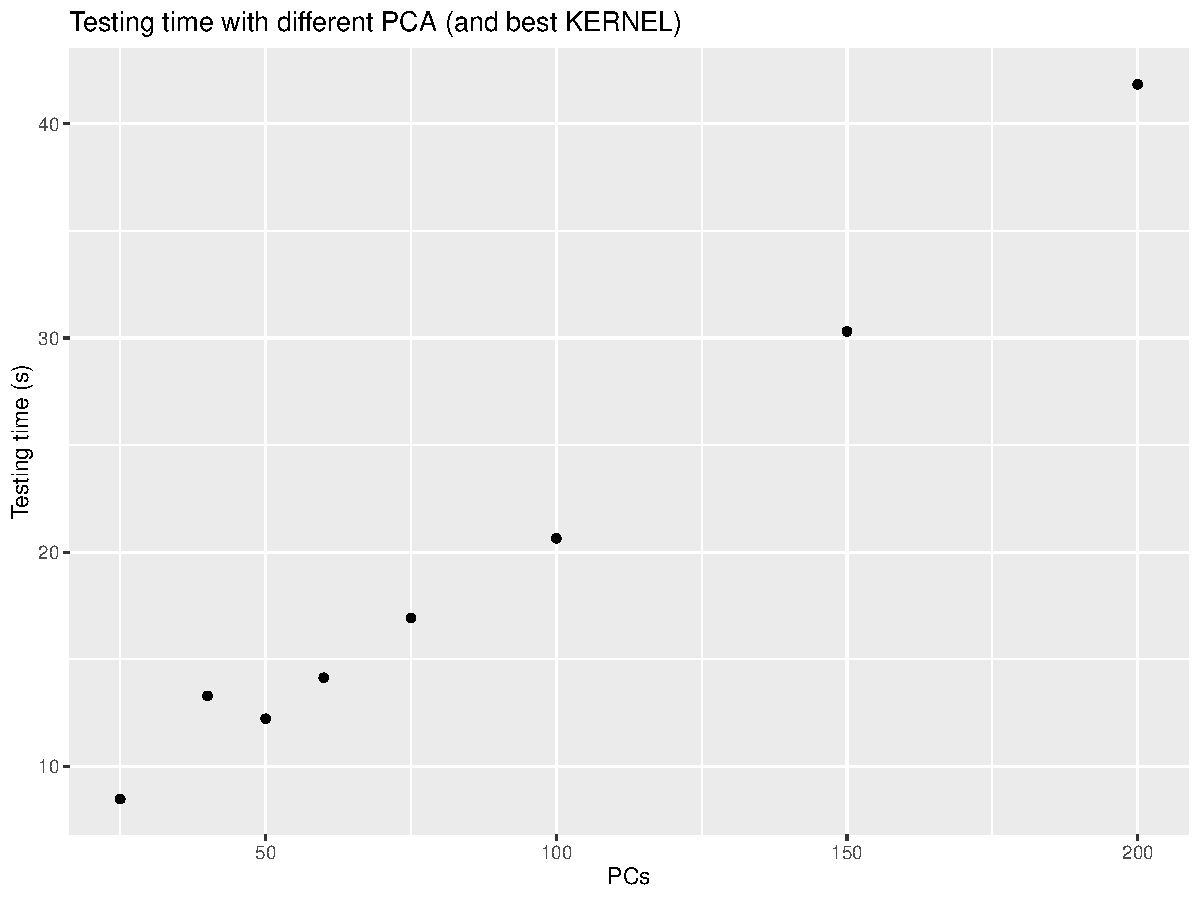
\includegraphics[width=0.3201\linewidth]{finalProject/SVM/Images_small/AllIn_Testing_PCA.pdf}}\quad   

    \subfloat[][]{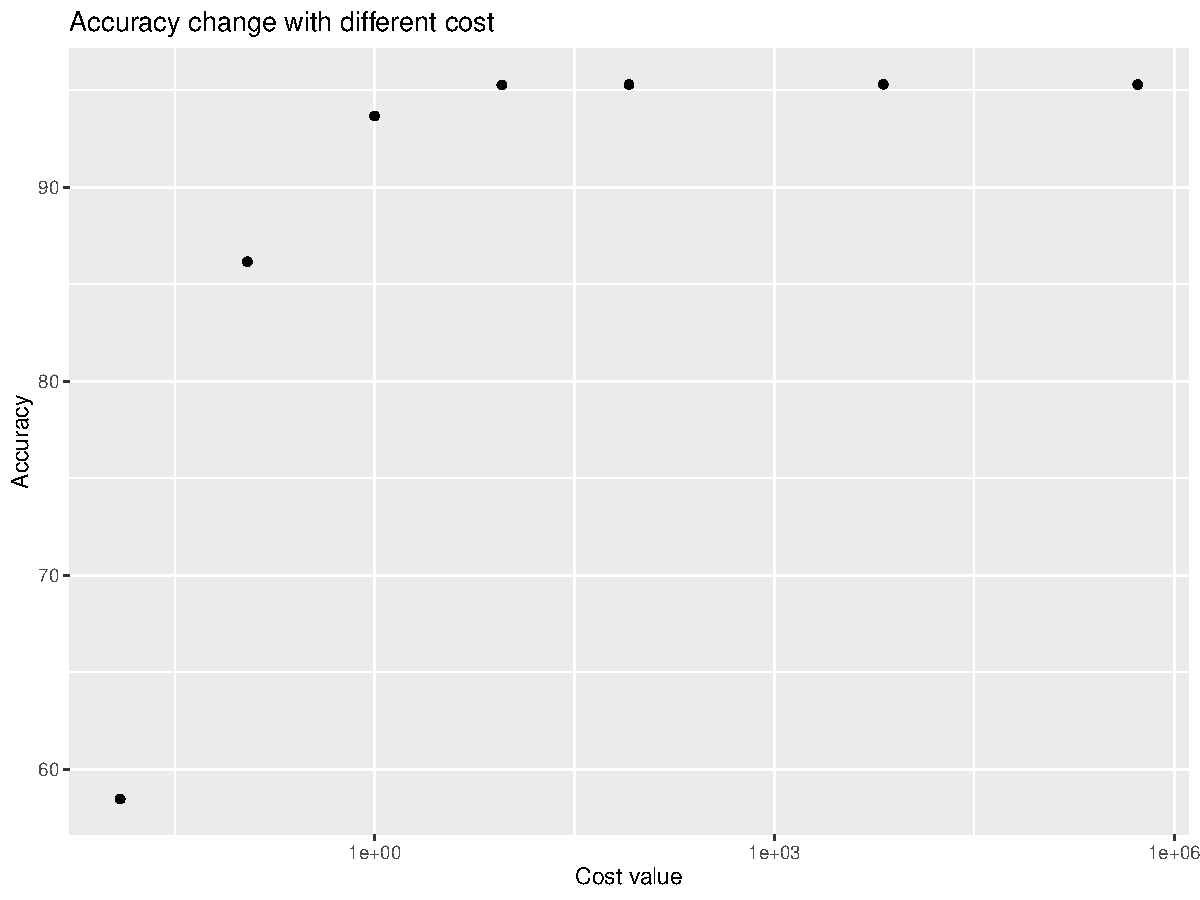
\includegraphics[width=0.3201\linewidth]{finalProject/SVM/Images_small/AllIn_Accuracy_Cost.pdf}}\quad
    \subfloat[][]{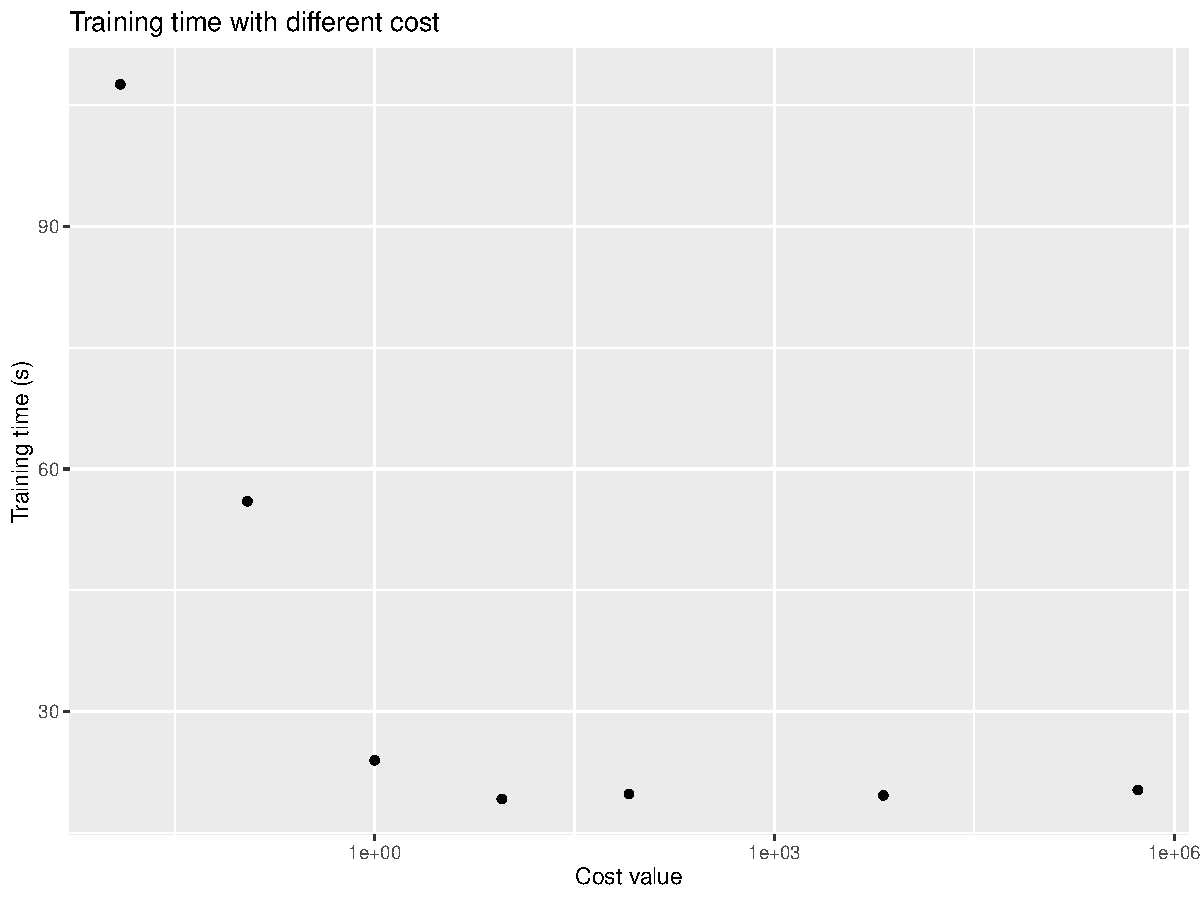
\includegraphics[width=0.3201\linewidth]{finalProject/SVM/Images_small/AllIn_Training_Cost.pdf}}\quad
    \subfloat[][]{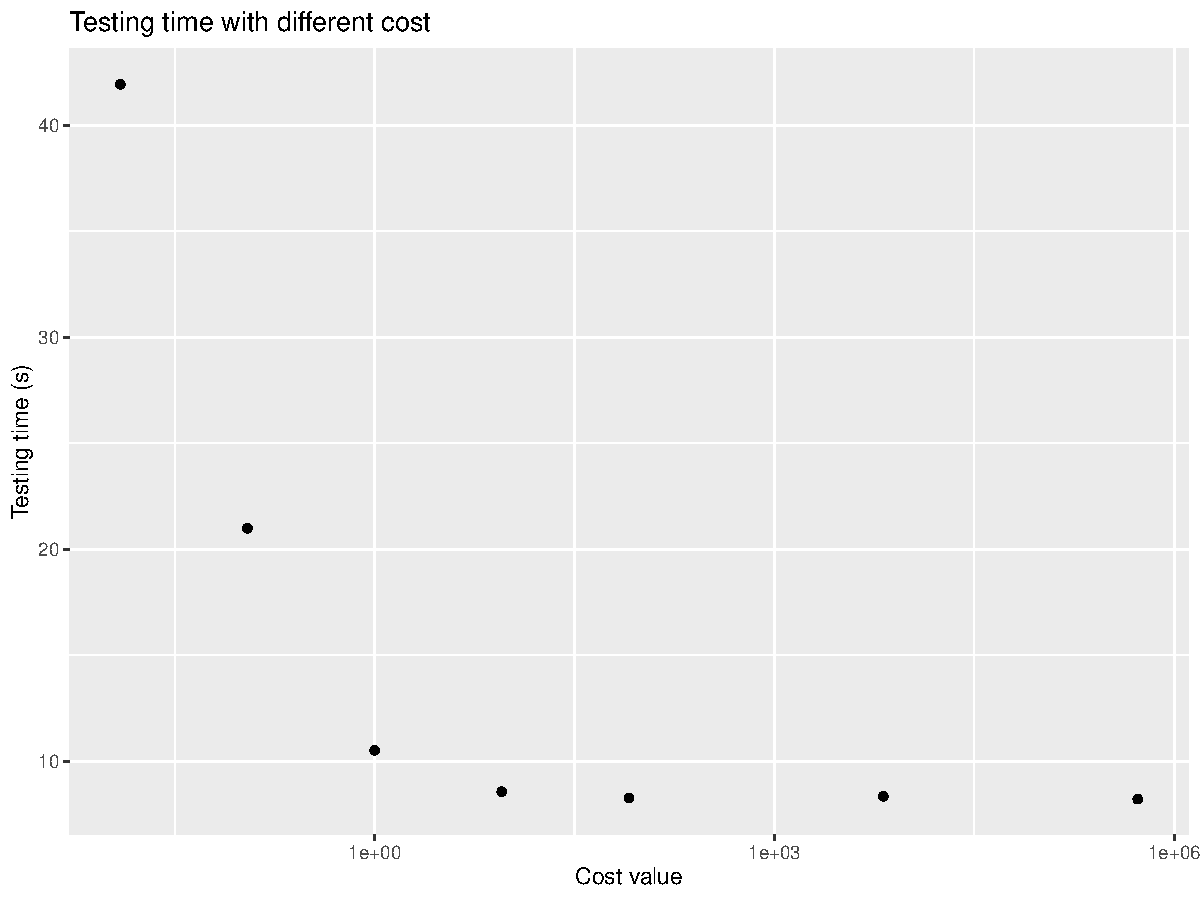
\includegraphics[width=0.3201\linewidth]{finalProject/SVM/Images_small/AllIn_Testing_Cost.pdf}}\quad

    \caption{
        \color{maxim}
        Accuracy and runtime results of the hyperparameter for "All-in" dataset; \\ 
        (a,b,c) Kernel accuracy, training time and testing time, respectively; (d,e,f) PCA accuracy, training time and testing time, respectively; (g,h,i) Cost accuracy, training time and testing time, respectively;
    }
    \label{fig:hyper:svm_param_allin}
\end{figure*}

\begin{figure*}[ht!]
    \centering

    \subfloat[][]{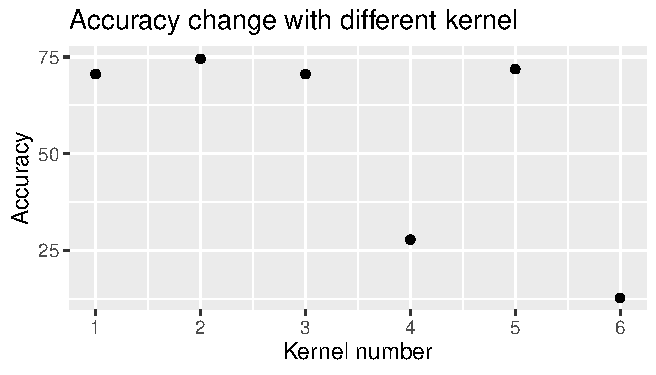
\includegraphics[width=0.3201\linewidth]{finalProject/SVM/Images_small/Disjunct_Accuracy_Kernel.pdf}}\quad
    \subfloat[][]{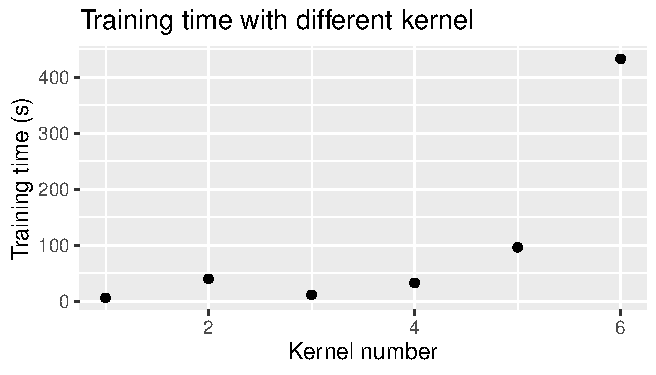
\includegraphics[width=0.3201\linewidth]{finalProject/SVM/Images_small/Disjunct_Training_Kernel.pdf}}\quad
    \subfloat[][]{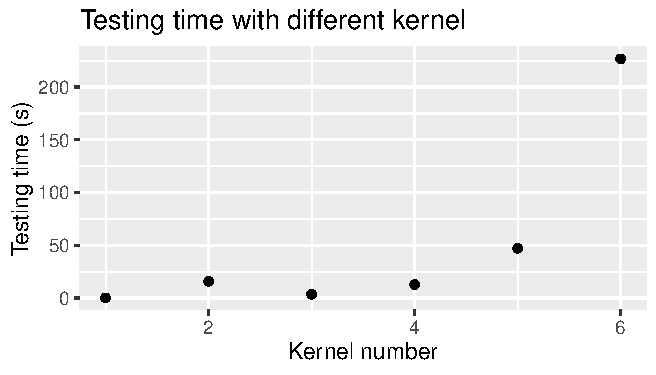
\includegraphics[width=0.3201\linewidth]{finalProject/SVM/Images_small/Disjunct_Testing_Kernel.pdf}}\quad
    
     \subfloat[][]{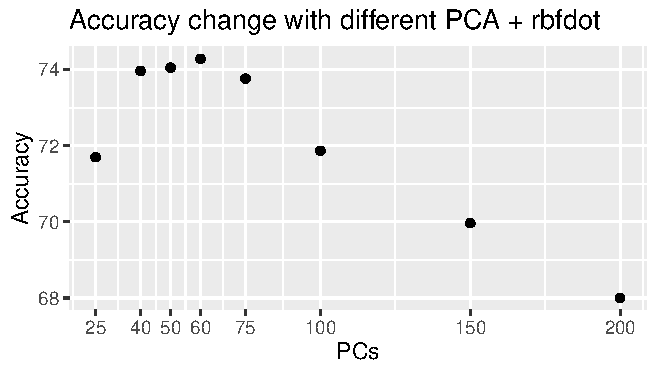
\includegraphics[width=0.3201\linewidth]{finalProject/SVM/Images_small/Disjunct_Accuracy_PCA.pdf}}\quad
    \subfloat[][]{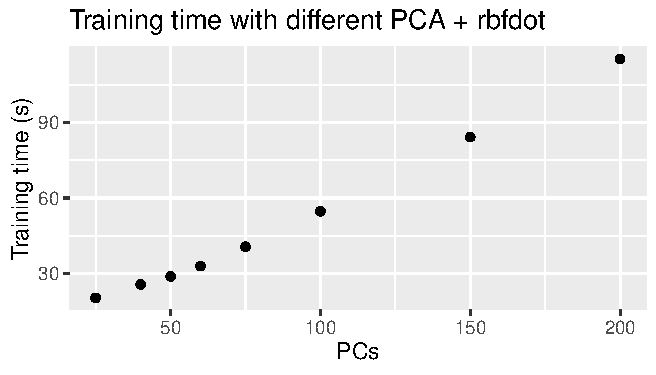
\includegraphics[width=0.3201\linewidth]{finalProject/SVM/Images_small/Disjunct_Training_PCA.pdf}}\quad
    \subfloat[][]{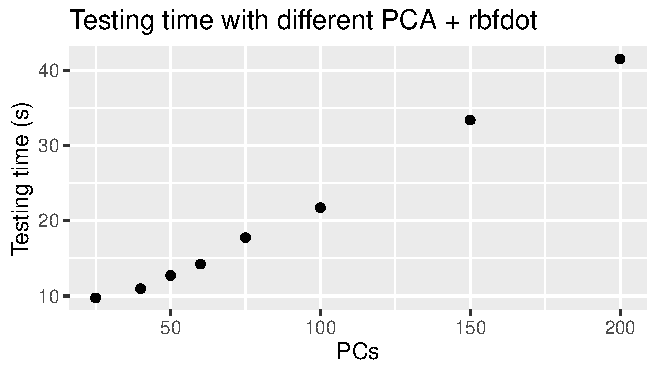
\includegraphics[width=0.3201\linewidth]{finalProject/SVM/Images_small/Disjunct_Testing_PCA.pdf}}\quad   

    \subfloat[][]{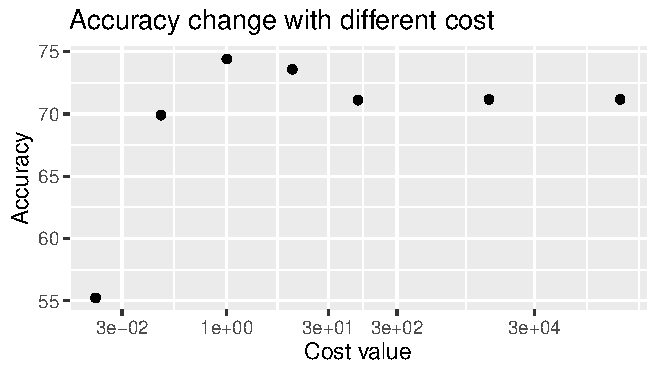
\includegraphics[width=0.3201\linewidth]{finalProject/SVM/Images_small/Disjunct_Accuracy_Cost.pdf}}\quad
    \subfloat[][]{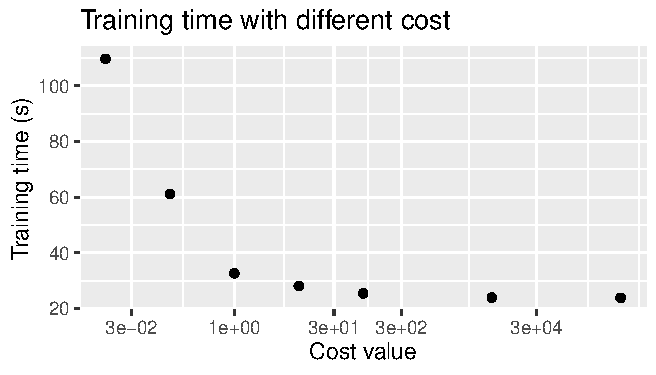
\includegraphics[width=0.3201\linewidth]{finalProject/SVM/Images_small/Disjunct_Training_Cost.pdf}}\quad
    \subfloat[][]{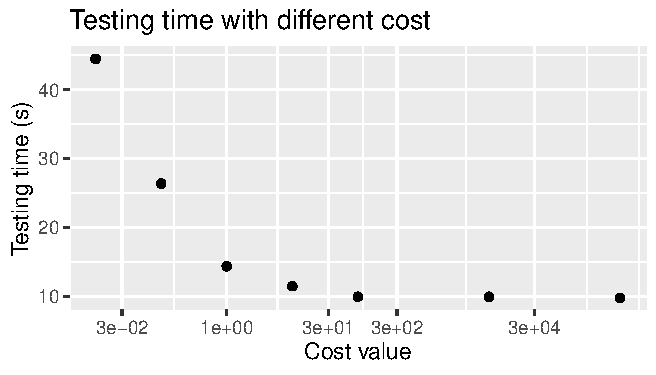
\includegraphics[width=0.3201\linewidth]{finalProject/SVM/Images_small/Disjunct_Testing_Cost.pdf}}\quad

    \caption{
        \color{maxim}
        Accuracy and runtime results of the hyperparameters for the "Disjunct" dataset; \\ 
        (a,b,c) Kernel accuracy, training time and testing time, respectively; (d,e,f) PCA accuracy, training time and testing time, respectively; (g,h,i) Cost accuracy, training time and testing time, respectively;
    }
    \label{fig:hyper:svm_param_allin}
\end{figure*}

\subsection{Hyper parameter Optimization for Support Vector Machine}\label{sec:hyper:svm}
\textcolor{maxim}{
    For the optimization of the SVM parameters we decided to use a small dataset of 8 people, 5 for the training set and 3 for the training set. Therefore, it reduced considerably the computation time. For the hyperparameters, we proceed as follow for both "All-in" and "Disjunct" dataset : first we checked all the different Kernel type, then we applied a Principal Component (PC) Analysis with different value of PCs followed by checking the effect of the cost function to our accuracy to finish by slightly modifying the kernel's parameter. We can see in \ref{table:gridParamSVM} the sequence's detail of our optimization for all the parameters.\\
    \subsubsection{Kernel Type $K_{type}$}
    Text here to explain the kernel type who got the best accuracy, why is it normal and stuff. \\
    \subsubsection{Amount of Principal Components $p$}
    Text here to explain the number of PC who got the best accuracy, why is it normal and the comparison between allin and disjunct. \\
    \subsubsection{Cost $C$}
    Text here to explain the Cost briefly and who got the best accuracy, why is it normal and the comparison between allin and disjunct. \\
    \subsubsection{Kernel Parameters $K_{par}$}
    Text here to explain the $K_{par}$ briefly and why we choose automatic.\\
    \subsubsection{Brief overview of the results}
    Text here to explain the results.\\
    }

% name, dataset split, dataset size, acc, train time, test time
% # Acc: 93.74706  Train time: 139.1029  Test time: 7.46046  # all in, with image wise norm
\begin{table*}[htbp]
    % \color{til}
    \caption{Intermediate Results after hyperparameter tuning}
    \begin{center}
    \begin{tabular}{|l|c|c|c|c|}
        \hline
        \textbf{Result name} & \textbf{Dataset split in students } & \textbf{Train time} & \textbf{Test time} & \textbf{Test accuracy} \\
        \hline
        Random Forest best gridsearch & disjunct 30 / 17 & 171 sec. & 3.26 sec. & 83.72\% \\
        \hline
        Random Forest + manual finetuned & disjunct 30 / 17 & 127 sec. & 7.27 sec. & 84.15\% \\
        \hline
        Random Forest + manual finetuned & all-in 30/17 & 129 sec. & 7.18 sec. & 93.97\% \\
        \hline
        Random Forest + manual finetuned + image wise min-max-norm & disjunct 30/17 & 138 sec. & 6.37 sec. & 85.68\% \\
        \hline
        Random Forest + manual finetuned + image wise min-max-norm & all-in 30/17 & 139 sec. & 7.46 sec. & 93.75\% \\
        \hline
        SVM (small dataset) & all-in 5/3 & 18.3 sec. & 9.24 sec. & 95.27\% \\
        \hline
        SVM (small dataset) & disjunct 5/3 & 34.7 sec. & 14.5 sec. & 74.23\% \\
        \hline
        SVM  & all-in 30/7 & 367 sec. & 127 sec. & 96.89\% \\
        \hline
        SVM  & disjunct 30/7 & 638 sec. & 205 sec. & 87.32\% \\
        \hline
        SVM + min-max-norm & all-in 30/7 & 234 sec. & 90.9 sec. & 97.20\% \\
        \hline
        SVM + min-max-norm & disjunct 30/7 & 368 sec. & 138 sec. & 89.04\% \\
        \hline

        
        %\multicolumn{5}{l}{$n$ size of training dataset, $p$ number of features used } \\
        % \multicolumn{4}{l}{$p$ number of features used } \\
        %\multicolumn{4}{l}{$n_{trees}$ number of various trees, $n_{sv}$ number of support vectors } \\
        % \multicolumn{4}{l}{$n_{sv}$ number of support vectors }
    \end{tabular}
    \label{table:timeIntermediateResults}
    \end{center}
\end{table*}

%problem: on a smaller set!!! => maybe say smaller set was 30people and use crossvalidation with 43 to 4 with bigger set => argue why 30people was not a problem, because of colab and kaggle we choose 30people and let it run over night
%explain grid search for: PCA, NTREE, MTRY, NODESIZE, SAMPSIZE
%=> manual hyperparam optimization (by interpreting grid search barplots)
%=> preprocess optimization (by using image wise min-max norm)
%(remeber: Give information about the computational time required.)


\section{Evaluation}
%Do a proper cross validation and indicate also mean and variances for all problems. Describe results on test and training set and reflect on overfitting. 
%(remember: Give information about the computational time required.)
%(remember: Analyze the results and give proper explanations)
\textcolor{baptiste}{In machine learning, the first thought when a given model gives a satisfying result is to conclude that this model is working and to apply it to other similar situations. However, when the model gives one satisfying result, it does not necessarily mean that it will work for other situations or even when considering other training and test sets of the same dataset. To make sure that all the important information and patterns of the data is picked up correctly, we need to do more testing than a single random training and test set in the dataset.}

\textcolor{baptiste}{To have an efficient machine learning model, it needs to be accurate on datasets it has never seen before. To make sure of that, we use what is called Cross Validation. It consists on taking a part of the dataset we are working on to train the model and the remaining part to test it as the data the model has never seen before.
A good way to be really sure that the model is accurate is to use K-Fold Cross Validation. It consists in separating the dataset in K subsets and to use each subset as the test set while the other subsets are the training set. 
}


\textcolor{baptiste}{The main problems when testing a machine learning model are underfitting and overfitting. Underfitting occurs when the model does not have enough parameters to fit and classify the data correctly. It shows when the training validation errors are high. It means that the model did not learn enough from the training set and needs to be made more complex in order to pick up enough parameters.}

\textcolor{baptiste}{Overfitting, on the other hand, is when the model has too many parameters. It shows when the training error is very low but the accuracy on unseen data is very poor. The model picked up too many parameters or parameters that are very specific to the training set and is not able to recognize objects in unseen data. In order to fix this issue, the model needs to be regulated and some parameters need to be removed.}

\textcolor{baptiste}{These issues show that machine learning is not as straight forward as it may seem: the more parameters we take into account does not necessarily mean that the model will perform better. There is a balance that needs to be achieved.
}




\subsection{Random Forest}

\textcolor{baptiste}{For the Random Forest model, we are using a 10-folds cross validation. In order to have the sets containing only an exact number of people, we are going to work with 40 people instead of the 47 available in the full dataset.}

\textcolor{baptiste}{The results are in the first two columns of Table \ref{table:CV_RF_results} and in Fig. \ref{fig:hyper:cv_RF}}

\begin{table*}[htbp]
    \color{baptiste}
    \caption{\color{baptiste}Cross Validation results for Random Forest model}
    \begin{center}
    \begin{tabular}{|l|c|c|c|c|}
        \hline
        \textbf{} & \textbf{Random Forest "Disjunct"} & \textbf{Random Forest "All Persons In"} & \textbf{SVM "Disjunct"} & \textbf{SVM "All Persons In"}\\
        \hline
        Average accuracy & 94.85\% & 94.78\% & 96.9\% & 97.7\% \\
        \hline
        Variance & 0.024 & 0.079 & 0.012 & 0.011 \\
        \hline
        Average training error & 0.025\% & 0.024\% & 1.86\% & 0.29\% \\
        \hline
        Average training time & 217.5s & 260.1s & 571.3s & 298.0s \\
        \hline
        Average test time & 2.5s & 3.0s & 93.7s & 45.8s \\
        \hline
    \end{tabular}
    \label{table:CV_results}
    \end{center}
\end{table*}
%=> use 10 fold crossvalidation with 43 to 4 with bigger set

%(remeber: Give information about the computational time required.)
%(remeber: Analyze the results and give proper explanations)

\begin{figure*}[ht!]
    \centering

    \subfloat[][]{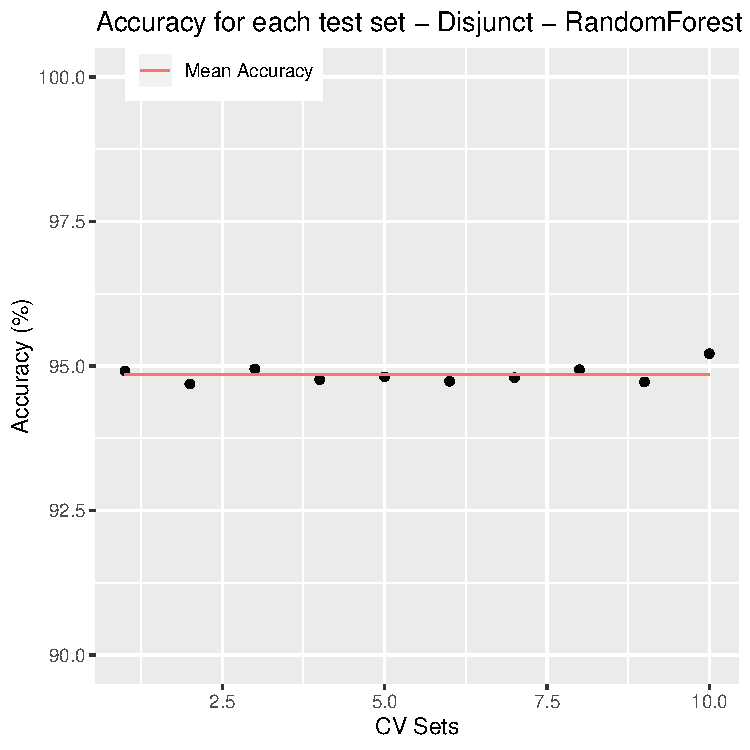
\includegraphics[width=0.3201\linewidth]{finalProject/CrossValidation/Accs_D_RF.pdf}}\quad
    \subfloat[][]{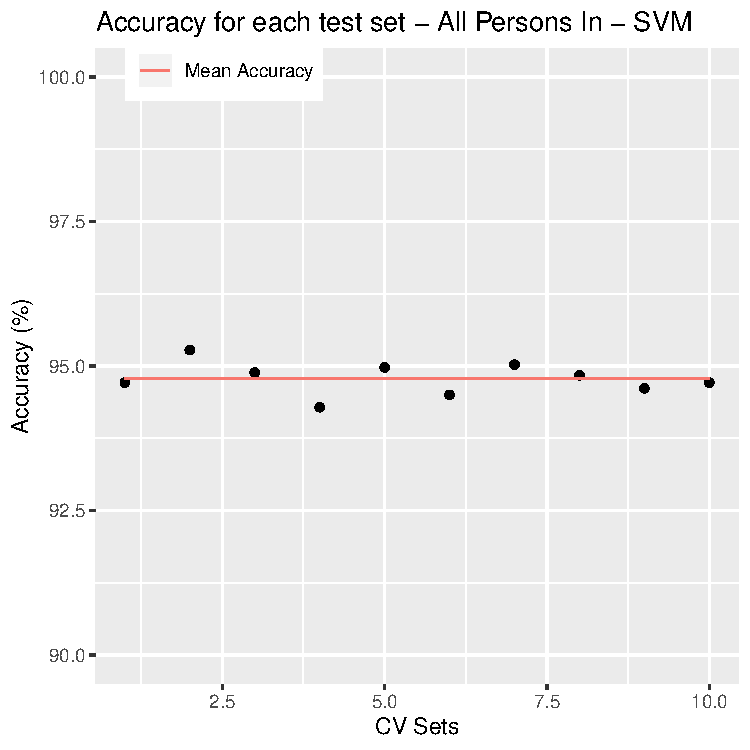
\includegraphics[width=0.3201\linewidth]{finalProject/CrossValidation/Accs_API_RF.pdf}}\quad
    
    \subfloat[][]{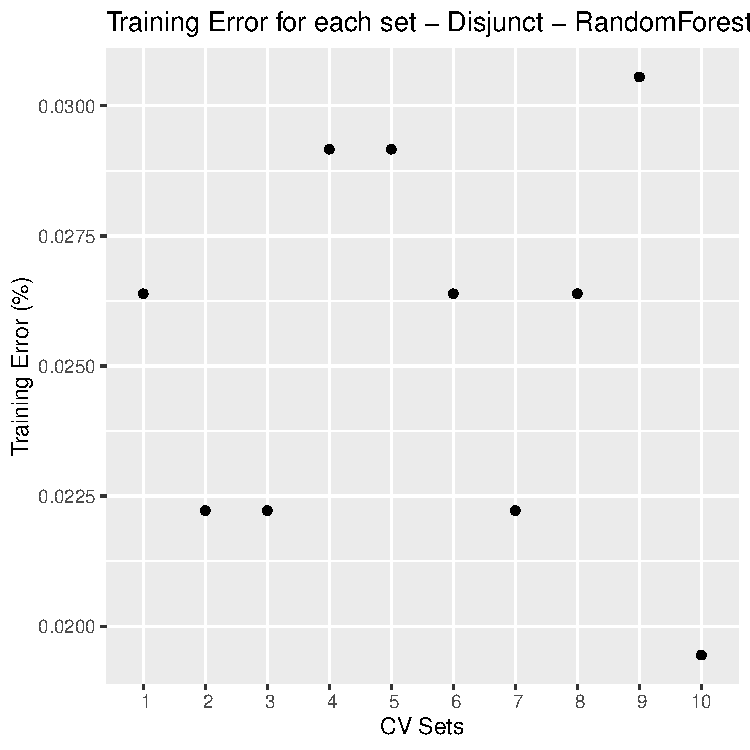
\includegraphics[width=0.3201\linewidth]{finalProject/CrossValidation/Terr_D_RF.pdf}}\quad
    \subfloat[][]{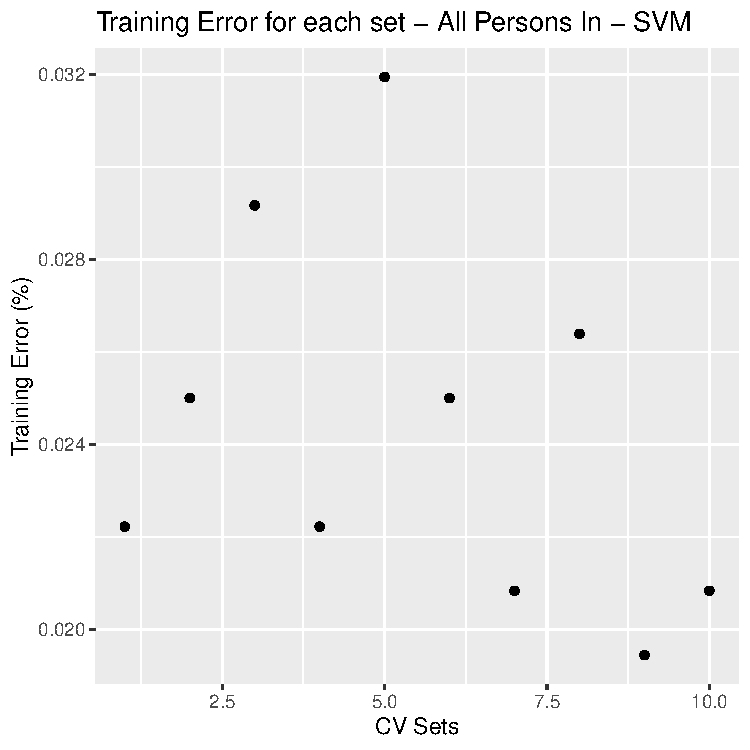
\includegraphics[width=0.3201\linewidth]{finalProject/CrossValidation/Terr_API_RF.pdf}}\quad

    \caption{
        \color{baptiste}
        Accuracy and training error for the subsets in the cross validation of the Random Forest model \\ 
        (a,b) Accuracy for "Disjunct" dataset and for "All Persons In" dataset respectively;
        (c,d) Training errors for "Disjunct" dataset and for "All Persons In" dataset respectively
    }
    \label{fig:hyper:cv_RF}
\end{figure*}

\subsection{Support Vector Machine}
\textcolor{baptiste}{For the SVM model, we only used 5 folds because of the runtimes of such models, that is meant to be more precise than Random Forest but also takes more time to compute.}

\textcolor{baptiste}{For the same reason that we used the data from 40 people for the Random Forest, we are going to use 45 people for SVM.
}

\textcolor{baptiste}{The results are in the last two columns of Table \ref{table:CV_results} and in Fig. \ref{fig:hyper:cv_SVM}}

\begin{figure*}[ht!]
    \centering

    \subfloat[][]{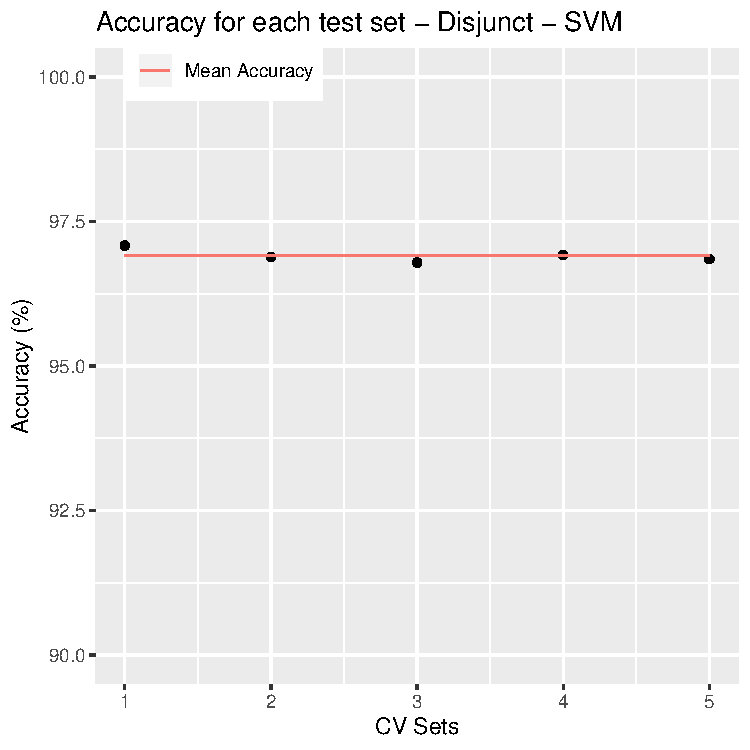
\includegraphics[width=0.3201\linewidth]{finalProject/CrossValidation/Accs_D_SVM.pdf}}\quad
    \subfloat[][]{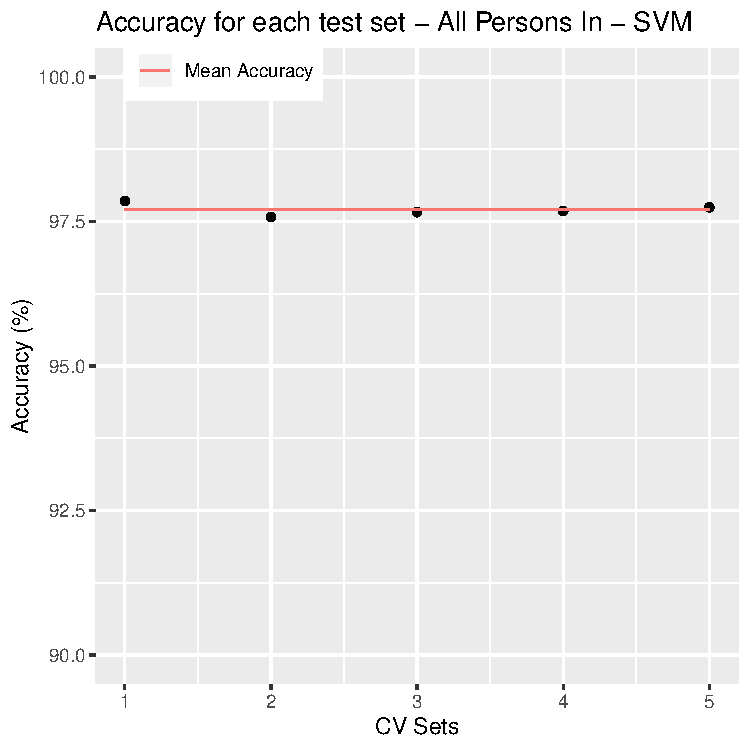
\includegraphics[width=0.3201\linewidth]{finalProject/CrossValidation/Accs_API_SVM.pdf}}\quad
    
    \subfloat[][]{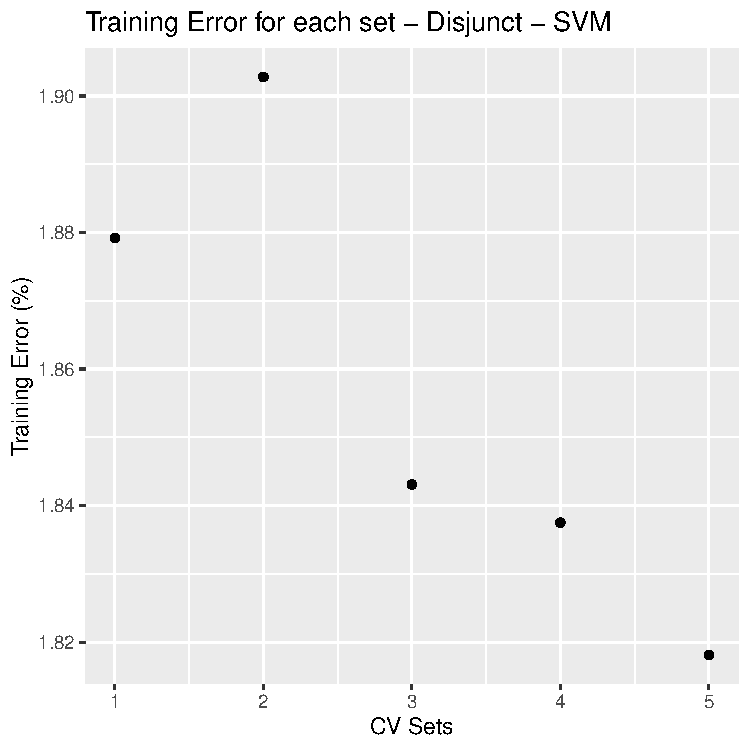
\includegraphics[width=0.3201\linewidth]{finalProject/CrossValidation/Terr_D_SVM.pdf}}\quad
    \subfloat[][]{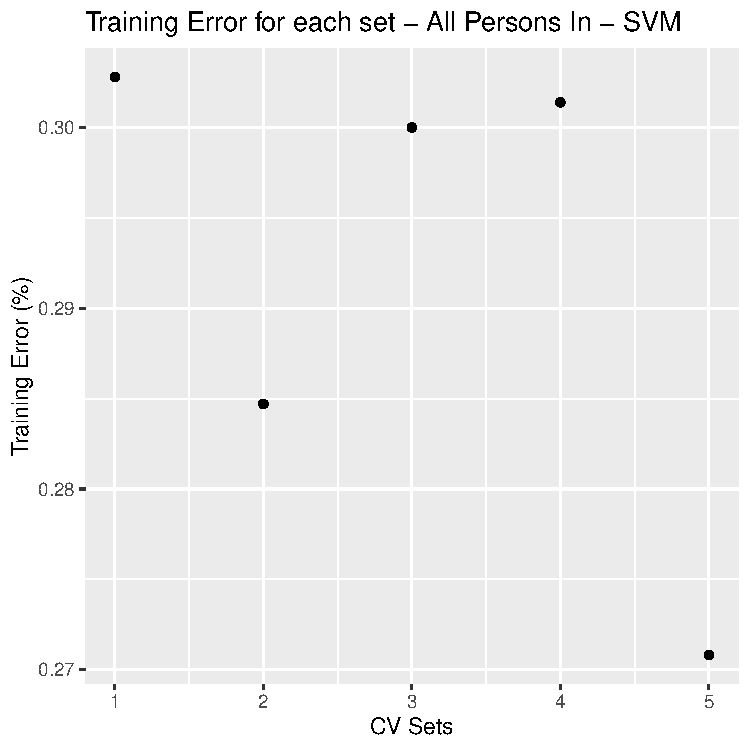
\includegraphics[width=0.3201\linewidth]{finalProject/CrossValidation/Terr_API_SVM.pdf}}\quad

    \caption{
        \color{baptiste}
        Accuracy and training error for the subsets in the cross validation of the Support Vector Machine model \\ 
        (a,b) Accuracy for "Disjunct" dataset and for "All Persons In" dataset respectively;
        (c,d) Training errors for "Disjunct" dataset and for "All Persons In" dataset respectively
    }
    \label{fig:hyper:cv_SVM}
\end{figure*}

\subsection{Results interpretation}

\textcolor{baptiste}{In all these situations we have a good training error and a good accuracy on unseen data with low variance so there is neither overfitting nor underfitting. Both the models we worked on are accurate and passed the cross validation test.}

\textcolor{baptiste}{As mentioned at the beginning, we can see by the results of the cross validation that there is one model that is relatively fast (Random Forest) and one that is more accurate but takes more time (SVM)}

\section{Future Work}
Give an indication what could be further improved. 

optimize Random forest model also on corner dataset and see how it works


% \begin{thebibliography}{00}
% \end{thebibliography}

\end{document}
